\documentclass[sigconf]{acmart}
\usepackage{lipsum}

% Local Commands
\newcommand{\ucscaffil}{\affiliation{\institution{University of California, Santa Cruz}\streetaddress{1156 High St - 95064}\city{Santa Cruz, CA}\country{U.S.A.}}}

\newcommand{\putgraphic}[3]{
\begin{figure}[h]
	\centering
	\includegraphics[width=\linewidth]{#1}
	\caption{#2}
	\Description{#3}
\end{figure}
}

% Document Configuration
\setcopyright{acmcopyright}
\copyrightyear{2019}
\acmYear{N/A}

\acmConference[Santa Cruz '19]{UC Santa Cruz '19: CMPM 163, Spring Quarter 2019}{June 01--13, 2019}{Santa Cruz, CA}
\acmBooktitle{UC Santa Cruz '19: CMPM 163 Final Project, June 01--13, 2019, Santa Cruz, CA}
\acmPrice{0.00}
\acmISBN{?????????}

\begin{document}

% TITLE CONFIGURATION
\title{VFX Demonstration: Close Encounter of the Second Kind}

\author{Anthony Medina}
\authornote{ROLE}
\email{amedin12@ucsc.edu}
\ucscaffil

\author{Jan Yu}
\authornote{ROLE}
\email{jyu92@ucsc.edu}
\ucscaffil

\author{Malcolm Riley}
\authornote{ROLE}
\email{masriley@ucsc.edu}
\ucscaffil

\renewcommand{\shortauthors}{Medina, Yu, and Riley}

\begin{abstract}
	\lipsum[1]
\end{abstract}

\begin{CCSXML}
<ccs2012>
	<concept>
		<concept_id>10010147.10010341</concept_id>
		<concept_desc>Computing methodologies~Modeling and simulation</concept_desc>	
		<concept_significance>500</concept_significance>
	</concept>
	<concept>
		<concept_id>10003120.10003145</concept_id>
		<concept_desc>Human-centered computing~Visualization</concept_desc>
		<concept_significance>500</concept_significance>
	</concept>
		<concept>
		<concept_id>10003120.10003121</concept_id>
		<concept_desc>Human-centered computing~Human computer interaction (HCI)</concept_desc>
		<concept_significance>100</concept_significance>
	</concept>
</ccs2012>
\end{CCSXML}

\ccsdesc[500]{Computing methodologies~Modeling and simulation}
\ccsdesc[500]{Human-centered computing~Visualization}
\ccsdesc[100]{Human-centered computing~Human computer interaction (HCI)}

\keywords{keywords,keywords,keywords}

%\begin{teaserfigure}
%	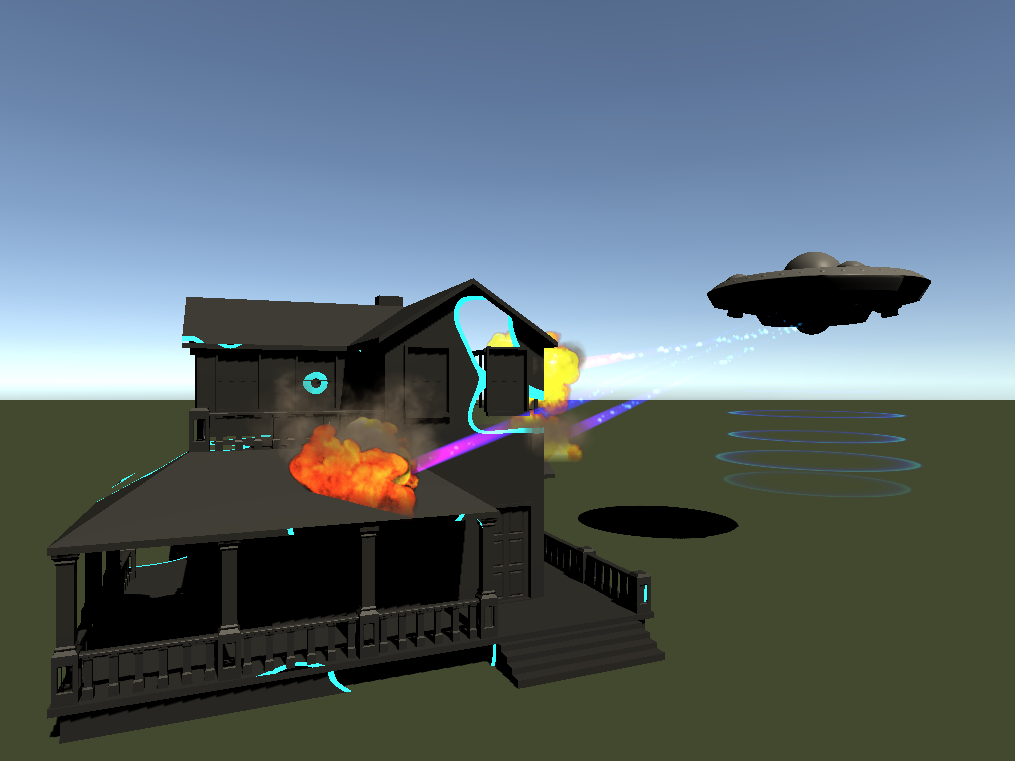
\includegraphics[width=\textwidth]{images\teaser}
%	\caption{CAPTION}
%	\Description{DESCRIPTION}
%	\label{fig:teaser}
%\end{teaserfigure}

% TITLE
\maketitle

% INTRODUCTION
\section{Introduction}
\lipsum[1]

\section{Explosion VFX}
\textit{Written by Anthony Medina.\quad}
\input{anthony-explosion.txt}

\section{House Dissolve VFX}
\textit{Written by Jan Yu.\quad}
\input{jan-dissolve.txt}

\section{UFO VFX}
\textit{Written by Malcolm Riley.\quad}
The primary focus of my visual-effects efforts was in the implementation of the UFO's energy weapon effects.
\putgraphic{plasmabolt}{The primary energy projectile effect.}{A close view of the UFO's primary energy projectile effect.}
There are four components to this effect: A modified rim shader applied to an oblong mesh forms the primary mass of the projectile, a considerably simpler transparent shader applied to a hemispherical mesh form the shockwave effect, and two simple particle systems form the trail and sparkles, respectively. The implementation of the latter two effects were trivial; being performed using Unity's built-in unlit particle shaders they will not be discussed in depth. Likewise, various other visual effects tasks were performed in the creation of this scene and will be discussed briefly in the ``Miscellaneous Effects'' section.

\subsection{Modified Rim Shader}
To add visual interest to the main mass of the energy projectile, a modified rim shader was used. As with any rim shader, the primary driving operation is the dot product of the normalized surface normal with the normalized view vector. However, it became desirable to modify this result by adding noise and an intensity factor.

The noise-enhanced rim incidence is thus given by the expression:

\begin{figure}[h]
	\centering
	\[
		R = (\mathbf{\hat{I}_N} \cdot \mathbf{\hat{I}_V})^k \times T^j
	\]
	\caption{Rim incidence vector equation.}
	\Description{The expression used to calculate the rim incidence vector.}
\end{figure}

Where $\mathbf{\hat{I}_N}$ is the normalized surface normal, $\mathbf{\hat{I}_V}$ is the normalized view vector, $k$ is an arbitrary ``Rim Intensity'' factor, $T$ is the noise texture sample color, and $j$ is another arbitrary intensity factor.

In CG, this calculation is performed as follows:

\begin{figure}[h]
	\begin{verbatim}
		pow(dot(input.normal, input.view), _RimIntensity)
	\end{verbatim}
	\begin{verbatim}
		* pow(noise, 1 - _NoiseIntensity)
	\end{verbatim}
	\caption{CG code for the rim incidence vector calculation.}{The expression used to calculate the noise-enhanced rim incidence vector, in CG code.}
\end{figure}



\subsection{Simple Transparent Shader}

\subsection{Miscellaneous Effects}

%\begin{figure}[h]
%	\centering
%	\includegraphics[width=\linewidth]{images/figure}
%	\caption{1907 Franklin Model D roadster. Photograph by Harris \& Ewing, Inc. [Public domain], via Wikimedia Commons. (\url{https://goo.gl/VLCRBB}).}
%	\Description{The 1907 Franklin Model D roadster.}
%\end{figure}

\end{document}